\documentclass[a4paper]{article}
\usepackage[a4paper,margin=0mm]{geometry}
\usepackage{fontspec}
\usepackage{unicode-math}
\usepackage{tikz}
\usepackage[table]{xcolor}
\usepackage[absolute]{textpos}
\usepackage{array}
\usepackage{multirow}

\setmainfont{Libertinus Serif}
\setsansfont{Libertinus Sans}
\setmathfont{Libertinus Math}

\definecolor{accent}{HTML}{0F6A52}
\definecolor{badge}{HTML}{A9CFC2}
\definecolor{ink}{HTML}{2A2E30}

\setlength{\TPHorizModule}{1mm}
\setlength{\TPVertModule}{1mm}
\setlength{\parindent}{0pt}
\setlength{\parskip}{0pt}
\emergencystretch=3em
\abovedisplayskip=4pt plus 2pt minus 2pt \belowdisplayskip=4pt plus 2pt minus 2pt \abovedisplayshortskip=2pt \belowdisplayshortskip=2pt
\pagestyle{empty}

\newcommand{\LCOL}{16mm}
\newcommand{\RCOL}{111mm}
\newcommand{\COLW}{83mm}

\newcommand{\topicheader}[2]{%
\begin{textblock*}{194mm}(16mm,10mm)
\begin{tikzpicture}
\node[fill=accent,text=white,font=\sffamily\bfseries\fontsize{13}{13}\selectfont,
      minimum width=9mm,minimum height=9mm,inner sep=0pt] at (4.5mm,-4.5mm) {#1};
\node[font=\sffamily\bfseries\fontsize{15}{16}\selectfont,text=ink,anchor=west] at (12mm,-4.5mm) {#2};
\end{tikzpicture}
\end{textblock*}
\begin{textblock*}{194mm}(16mm,22.5mm)

\begin{tikzpicture}
\fill[accent] (0,0) rectangle (194mm,0.5mm);
\end{tikzpicture}
\end{textblock*}
}

\newcommand{\pagefooter}[1]{%
\begin{textblock*}{194mm}(8mm,286.41mm)
  
\begin{tikzpicture}
    \fill[accent] (0,0) rectangle (194mm,0.6mm);
  \end{tikzpicture}
\end{textblock*}
\begin{textblock*}{63.59mm}(8mm,288.27mm)
  {\sffamily\bfseries\color{accent}\fontsize{13}{16}\selectfont SAT 1200+}
\end{textblock*}
\begin{textblock*}{10mm}(188mm,288.27mm)
  \centering{\sffamily\color{accent}\fontsize{14}{16}\selectfont #1}
\end{textblock*}
}

\newcommand{\colrule}[2]{%
\begin{textblock*}{1mm}(105mm,#1mm)
\begin{tikzpicture}
\draw[black!65,line width=0.5pt] (0,0) -- (0,#2mm);
\end{tikzpicture}
\end{textblock*}
}

\newcommand{\setkicker}[2]{%
{\sffamily\bfseries\fontsize{12}{14}\selectfont #1.}\ {\itshape\fontsize{11}{14}\selectfont\color{black!75} #2}\par\vspace{2mm}%
}

\setlength{\fboxsep}{1.4pt}
\setlength{\fboxrule}{0.5pt}
\newcommand{\pnum}[1]{\fcolorbox{ink}{white}{\sffamily\bfseries\fontsize{8}{8}\selectfont #1}~}

% ---- SAT-style multiple-choice block (2x2 grid of short choices) ----
\newcommand{\satq}[6]{%
\noindent\pnum{#1} #2\par\nobreak\vspace{2mm}%
\noindent\hspace*{7mm}\begin{tabular}[t]{@{}p{32mm}p{32mm}@{}}
(A) #3 & (B) #4 \\[2mm]
(C) #5 & (D) #6 \\
\end{tabular}\par\vspace{5.5mm}%
}

% ---- stacked choices for long ones ----
\newcommand{\satqw}[6]{%
\noindent\pnum{#1} #2\par\nobreak\vspace{2mm}%
\noindent\hspace*{7mm}(A) #3\par\vspace{1.6mm}%
\noindent\hspace*{7mm}(B) #4\par\vspace{1.6mm}%
\noindent\hspace*{7mm}(C) #5\par\vspace{1.6mm}%
\noindent\hspace*{7mm}(D) #6\par\vspace{5.5mm}%
}

% ---- student-produced response (grid-in) ----
\newcommand{\satg}[2]{%
\noindent\pnum{#1} {\sffamily\bfseries\fontsize{7}{8}\selectfont\color{accent}GRID-IN}\ #2\par\nobreak\vspace{2.5mm}%
\noindent\hspace*{7mm}{\sffamily\fontsize{8.5}{10}\selectfont Answer:}\ \rule[-1.2mm]{28mm}{0.4pt}\par\vspace{5.5mm}%
}

% ---- worked-solution entry ----
\newcommand{\solitem}[4]{%
\noindent\pnum{#1} {\bfseries #2}\ —\ #3\ {\itshape\color{accent}[#4]}\par\vspace{2.1mm}%
}

\usetikzlibrary{arrows.meta}
\newsavebox{\figsave}
\newcommand{\figbox}[1]{\par\vspace{1.8mm}\sbox{\figsave}{#1}\noindent\hfill\ifdim\wd\figsave>\hsize\resizebox{\hsize}{!}{\usebox{\figsave}}\else\usebox{\figsave}\fi\hfill\null\par\vspace{0.8mm}}
\arrayrulecolor{accent}
\setlength{\arrayrulewidth}{0.7pt}
\renewcommand{\arraystretch}{1.3}

\usepackage{multicol}
\usepackage{fancyhdr}
\usepackage{needspace}
\newcommand{\pgoff}{0}
\renewcommand{\solitem}[4]{\noindent\parbox[t]{\linewidth}{\raggedright\pnum{#1} {\bfseries #2}\ ---\ #3\ {\itshape\color{accent}[#4]}}\par\vspace{3.6mm}}
\newcommand{\solkicker}[2]{\Needspace{38mm}\vspace{1.5mm}{\sffamily\bfseries\fontsize{12.5}{15}\selectfont #1.}\ {\itshape\fontsize{11}{14}\selectfont\color{black!75} #2}\par\vspace{3mm}}
\renewcommand{\satqw}[6]{%
\noindent\pnum{#1} #2\par\nobreak\vspace{2mm}%
\noindent\hangindent=13mm\hangafter=1\hspace*{7mm}(A)~#3\par\vspace{1.6mm}%
\noindent\hangindent=13mm\hangafter=1\hspace*{7mm}(B)~#4\par\vspace{1.6mm}%
\noindent\hangindent=13mm\hangafter=1\hspace*{7mm}(C)~#5\par\vspace{1.6mm}%
\noindent\hangindent=13mm\hangafter=1\hspace*{7mm}(D)~#6\par\vspace{5.5mm}%
}
\newcommand{\solkitem}[5]{\noindent\parbox[t]{\linewidth}{\vspace{1.5mm}{\sffamily\bfseries\fontsize{12.5}{15}\selectfont #1.}\ {\itshape\fontsize{11}{14}\selectfont\color{black!75} Worked solutions}\par\vspace{3mm}\raggedright\pnum{#2} {\bfseries #3}\ ---\ #4\ {\itshape\color{accent}[#5]}}\par\vspace{3.6mm}}
\fancypagestyle{solstyle}{\fancyhf{}\renewcommand{\headrulewidth}{0pt}\renewcommand{\footrulewidth}{0pt}%
 \fancyhead[L]{\topicheader{8}{Hard Circles, Area \& Volume}}%
 \fancyfoot[L]{\pagefooter{\the\numexpr\value{page}+\pgoff\relax}}}

\newwrite\mw \immediate\openout\mw=figmeas.txt
\begin{document}
\sbox{\figsave}{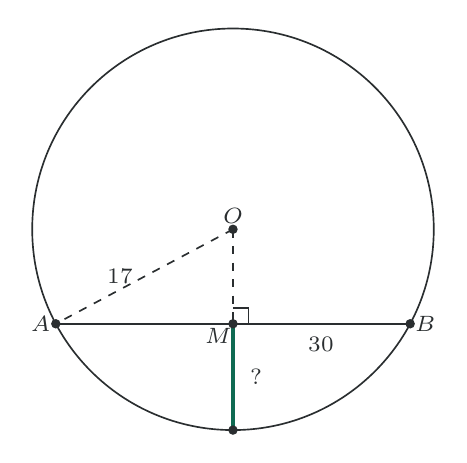
\begin{tikzpicture}[line width=0.6pt,ink,every node/.style={font=\footnotesize}]
\draw (0.000mm,0.000mm) circle (25.500mm);
\draw (-22.500mm,-12.000mm) -- (22.500mm,-12.000mm);
\draw[dashed] (0.000mm,0.000mm) -- (0.000mm,-12.000mm);
\draw[dashed] (0.000mm,0.000mm) -- (-22.500mm,-12.000mm);
\draw[accent,line width=1.4pt] (0.000mm,-12.000mm) -- (0.000mm,-25.500mm);
\draw[ink,line width=0.4pt] (0.000mm,-10.000mm) -- (2.000mm,-10.000mm) -- (2.000mm,-12.000mm);
\fill[ink] (0.000mm,0.000mm) circle (0.6mm); \node[above,inner sep=1.5pt] at (0.000mm,0.000mm) {$O$};
\fill[ink] (-22.500mm,-12.000mm) circle (0.6mm); \node[left,inner sep=1.5pt] at (-22.500mm,-12.000mm) {$A$};
\fill[ink] (22.500mm,-12.000mm) circle (0.6mm); \node[right,inner sep=1.5pt] at (22.500mm,-12.000mm) {$B$};
\fill[ink] (0.000mm,-12.000mm) circle (0.6mm); \node[below left,inner sep=1.5pt,xshift=0.5pt] at (0.000mm,-12.000mm) {$M$};
\fill[ink] (0.000mm,-25.500mm) circle (0.6mm);
\node[below=1pt] at (11.250mm,-12.000mm) {$30$};
\node[left=0.5pt] at (-11.250mm,-6.000mm) {$17$};
\node[right=1pt] at (0.600mm,-18.750mm) {$?$};
\end{tikzpicture}}\immediate\write\mw{sagitta \the\wd\figsave\space\the\ht\figsave\space\the\dp\figsave}
\sbox{\figsave}{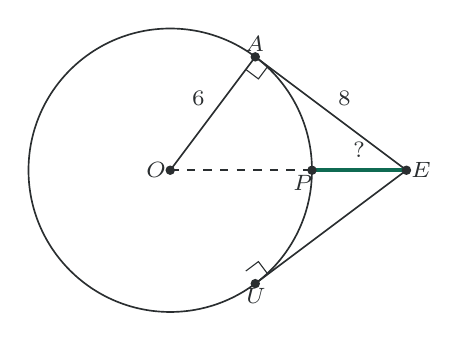
\begin{tikzpicture}[line width=0.6pt,ink,every node/.style={font=\footnotesize}]
\draw (0.000mm,0.000mm) circle (18.000mm);
\draw (0.000mm,0.000mm) -- (10.800mm,14.400mm) -- (30.000mm,0.000mm) -- (10.800mm,-14.400mm);
\draw[dashed] (0.000mm,0.000mm) -- (30.000mm,0.000mm);
\draw[accent,line width=1.4pt] (18.000mm,0.000mm) -- (30.000mm,0.000mm);
\draw[ink,line width=0.4pt] (9.600mm,12.800mm) -- (11.200mm,11.600mm) -- (12.400mm,13.200mm);
\draw[ink,line width=0.4pt] (9.600mm,-12.800mm) -- (11.200mm,-11.600mm) -- (12.400mm,-13.200mm);
\fill[ink] (0.000mm,0.000mm) circle (0.6mm); \node[left,inner sep=1.5pt] at (0.000mm,0.000mm) {$O$};
\fill[ink] (10.800mm,14.400mm) circle (0.6mm); \node[above,inner sep=1.5pt] at (10.800mm,14.400mm) {$A$};
\fill[ink] (10.800mm,-14.400mm) circle (0.6mm); \node[below,inner sep=1.5pt] at (10.800mm,-14.400mm) {$U$};
\fill[ink] (30.000mm,0.000mm) circle (0.6mm); \node[right,inner sep=1.5pt] at (30.000mm,0.000mm) {$E$};
\fill[ink] (18.000mm,0.000mm) circle (0.6mm); \node[below left,inner sep=1.5pt,xshift=1pt] at (18.000mm,0.000mm) {$P$};
\node[above left=-1pt] at (5.400mm,7.200mm) {$6$};
\node[above right=-1pt] at (20.400mm,7.200mm) {$8$};
\node[above=1pt] at (24.000mm,0.000mm) {$?$};
\end{tikzpicture}}\immediate\write\mw{kite \the\wd\figsave\space\the\ht\figsave\space\the\dp\figsave}
\sbox{\figsave}{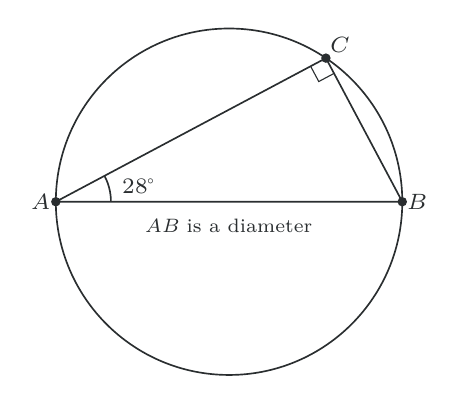
\begin{tikzpicture}[line width=0.6pt,ink,every node/.style={font=\footnotesize}]
\draw (0.000mm,0.000mm) circle (22.000mm);
\draw (-22.000mm,0.000mm) -- (22.000mm,0.000mm) -- (12.302mm,18.239mm) -- cycle;
\draw[ink,line width=0.4pt] (10.360mm,17.206mm) -- (11.393mm,15.264mm) -- (13.335mm,16.296mm);
\draw (-15.000mm,0.000mm) arc[start angle=0,end angle=28.000,radius=7mm];
\node[right] at (-14.800mm,1.900mm) {$28^\circ$};
\fill[ink] (-22.000mm,0.000mm) circle (0.6mm); \node[left,inner sep=1.5pt] at (-22.000mm,0.000mm) {$A$};
\fill[ink] (22.000mm,0.000mm) circle (0.6mm); \node[right,inner sep=1.5pt] at (22.000mm,0.000mm) {$B$};
\fill[ink] (12.302mm,18.239mm) circle (0.6mm); \node[above right,inner sep=1.5pt] at (12.302mm,18.239mm) {$C$};
\node[below=1pt] at (0.000mm,-0.500mm) {\scriptsize $AB$ is a diameter};
\end{tikzpicture}}\immediate\write\mw{semicircle \the\wd\figsave\space\the\ht\figsave\space\the\dp\figsave}
\sbox{\figsave}{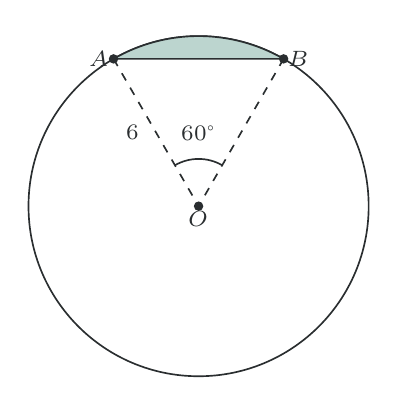
\begin{tikzpicture}[line width=0.6pt,ink,every node/.style={font=\footnotesize}]
\draw (0.000mm,0.000mm) circle (21.600mm);
\fill[accent!28] (10.800mm,18.706mm) arc[start angle=60.000,end angle=120.000,radius=21.600mm] -- cycle;
\draw (10.800mm,18.706mm) arc[start angle=60.000,end angle=120.000,radius=21.600mm] -- cycle;
\draw[dashed] (-10.800mm,18.706mm) -- (0.000mm,0.000mm) -- (10.800mm,18.706mm);
\draw (3.000mm,5.196mm) arc[start angle=60.000,end angle=120.000,radius=6mm];
\node at (0.000mm,9.200mm) {$60^\circ$};
\fill[ink] (0.000mm,0.000mm) circle (0.6mm); \node[below,inner sep=1.5pt] at (0.000mm,0.000mm) {$O$};
\fill[ink] (-10.800mm,18.706mm) circle (0.6mm); \node[left,inner sep=1.5pt] at (-10.800mm,18.706mm) {$A$};
\fill[ink] (10.800mm,18.706mm) circle (0.6mm); \node[right,inner sep=1.5pt] at (10.800mm,18.706mm) {$B$};
\node[left=1pt] at (-5.900mm,9.353mm) {$6$};
\end{tikzpicture}}\immediate\write\mw{segment \the\wd\figsave\space\the\ht\figsave\space\the\dp\figsave}
\sbox{\figsave}{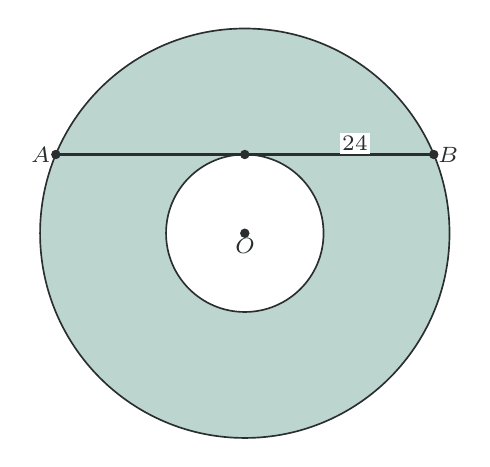
\begin{tikzpicture}[line width=0.6pt,ink,every node/.style={font=\footnotesize}]
\fill[accent!28,even odd rule] (0.000mm,0.000mm) circle (26.000mm) (0.000mm,0.000mm) circle (10.000mm);
\draw (0.000mm,0.000mm) circle (26.000mm); \draw (0.000mm,0.000mm) circle (10.000mm);
\draw[line width=0.9pt] (-24.000mm,10.000mm) -- (24.000mm,10.000mm);
\fill[ink] (0.000mm,0.000mm) circle (0.6mm); \node[below,inner sep=1.5pt] at (0.000mm,0.000mm) {$O$};
\fill[ink] (-24.000mm,10.000mm) circle (0.6mm); \node[left,inner sep=1.5pt] at (-24.000mm,10.000mm) {$A$};
\fill[ink] (24.000mm,10.000mm) circle (0.6mm); \node[right,inner sep=1.5pt] at (24.000mm,10.000mm) {$B$};
\fill[ink] (0.000mm,10.000mm) circle (0.6mm);
\node[above,fill=white,inner sep=1pt] at (14.000mm,10.000mm) {$24$};
\end{tikzpicture}}\immediate\write\mw{annulus \the\wd\figsave\space\the\ht\figsave\space\the\dp\figsave}
\sbox{\figsave}{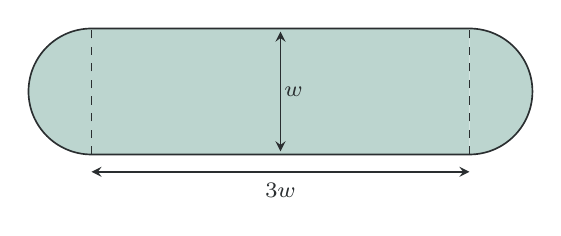
\begin{tikzpicture}[line width=0.6pt,ink,every node/.style={font=\footnotesize}]
\fill[accent!28] (0.000mm,0.000mm) rectangle (48.000mm,16.000mm);
\fill[accent!28] (48.000mm,0.000mm) arc[start angle=-90,end angle=90,radius=8.000mm] -- cycle;
\fill[accent!28] (0.000mm,0.000mm) arc[start angle=270,end angle=90,radius=8.000mm] -- cycle;
\draw (0.000mm,0.000mm) -- (48.000mm,0.000mm) arc[start angle=-90,end angle=90,radius=8.000mm] -- (0.000mm,16.000mm) arc[start angle=90,end angle=270,radius=8.000mm] -- cycle;
\draw[dashed] (0.000mm,0.000mm) -- (0.000mm,16.000mm); \draw[dashed] (48.000mm,0.000mm) -- (48.000mm,16.000mm);
\draw[<->,>=stealth] (24.000mm,0.400mm) -- (24.000mm,15.600mm) node[midway,right,inner sep=1pt] {$w$};
\draw[<->,>=stealth] (0.000mm,-2.200mm) -- (48.000mm,-2.200mm) node[midway,below=0.5pt] {$3w$};
\end{tikzpicture}}\immediate\write\mw{stadium \the\wd\figsave\space\the\ht\figsave\space\the\dp\figsave}
\sbox{\figsave}{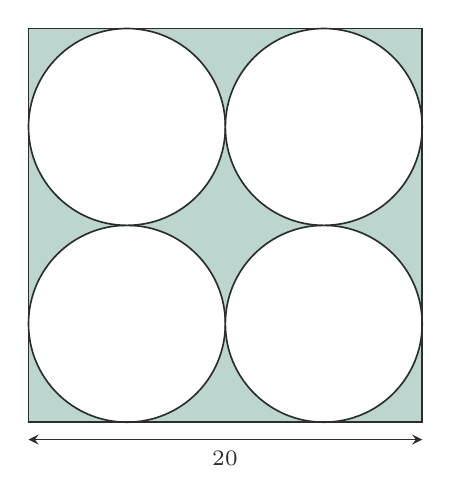
\begin{tikzpicture}[line width=0.6pt,ink,every node/.style={font=\footnotesize}]
\fill[accent!28] (0.000mm,0.000mm) rectangle (50.000mm,50.000mm);
\filldraw[fill=white] (12.500mm,12.500mm) circle (12.500mm);
\filldraw[fill=white] (12.500mm,37.500mm) circle (12.500mm);
\filldraw[fill=white] (37.500mm,12.500mm) circle (12.500mm);
\filldraw[fill=white] (37.500mm,37.500mm) circle (12.500mm);
\draw (0.000mm,0.000mm) rectangle (50.000mm,50.000mm);
\draw[<->,>=stealth] (0.000mm,-2.200mm) -- (50.000mm,-2.200mm) node[midway,below=0.5pt] {$20$};
\end{tikzpicture}}\immediate\write\mw{fourcircles \the\wd\figsave\space\the\ht\figsave\space\the\dp\figsave}
\sbox{\figsave}{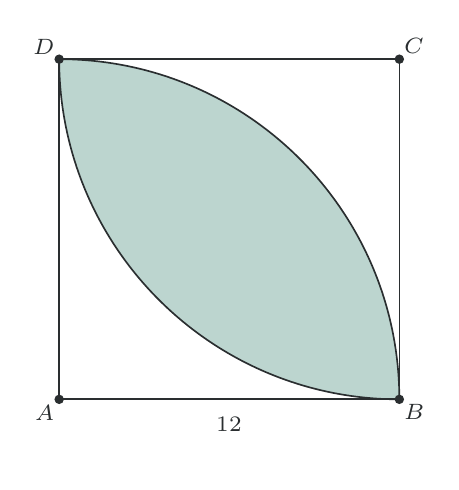
\begin{tikzpicture}[line width=0.6pt,ink,every node/.style={font=\footnotesize}]
\path[use as bounding box] (-4.000mm,-8.000mm) rectangle (47.200mm,47.200mm);
\begin{scope}\clip (0.000mm,0.000mm) circle (43.200mm); \fill[accent!28] (43.200mm,43.200mm) circle (43.200mm);\end{scope}
\draw (0.000mm,0.000mm) rectangle (43.200mm,43.200mm);
\draw (43.200mm,0.000mm) arc[start angle=0,end angle=90,radius=43.200mm];
\draw (0.000mm,43.200mm) arc[start angle=180,end angle=270,radius=43.200mm];
\fill[ink] (0.000mm,0.000mm) circle (0.6mm); \node[below left,inner sep=1.5pt] at (0.000mm,0.000mm) {$A$};
\fill[ink] (43.200mm,0.000mm) circle (0.6mm); \node[below right,inner sep=1.5pt] at (43.200mm,0.000mm) {$B$};
\fill[ink] (43.200mm,43.200mm) circle (0.6mm); \node[above right,inner sep=1.5pt] at (43.200mm,43.200mm) {$C$};
\fill[ink] (0.000mm,43.200mm) circle (0.6mm); \node[above left,inner sep=1.5pt] at (0.000mm,43.200mm) {$D$};
\node[below=1pt] at (21.600mm,-0.600mm) {$12$};
\end{tikzpicture}}\immediate\write\mw{lens \the\wd\figsave\space\the\ht\figsave\space\the\dp\figsave}
\sbox{\figsave}{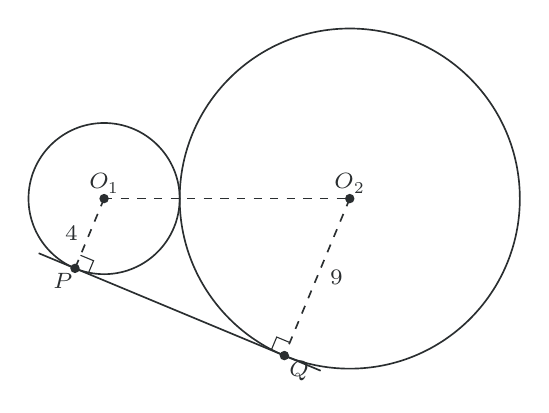
\begin{tikzpicture}[line width=0.6pt,ink,every node/.style={font=\footnotesize}]
\draw (0.000mm,0.000mm) circle (9.600mm); \draw (31.200mm,0.000mm) circle (21.600mm);
\draw (-8.308mm,-6.938mm) -- (27.508mm,-21.862mm);
\draw[dashed] (0.000mm,0.000mm) -- (-3.692mm,-8.862mm); \draw[dashed] (31.200mm,0.000mm) -- (22.892mm,-19.938mm);
\draw[dashed] (0.000mm,0.000mm) -- (31.200mm,0.000mm);
\draw[ink,line width=0.4pt] (-3.000mm,-7.200mm) -- (-1.338mm,-7.892mm) -- (-2.031mm,-9.554mm);
\draw[ink,line width=0.4pt] (23.585mm,-18.277mm) -- (21.923mm,-17.585mm) -- (21.231mm,-19.246mm);
\fill[ink] (0.000mm,0.000mm) circle (0.6mm); \node[above,inner sep=1.5pt] at (0.000mm,0.000mm) {$O_1$};
\fill[ink] (31.200mm,0.000mm) circle (0.6mm); \node[above,inner sep=1.5pt] at (31.200mm,0.000mm) {$O_2$};
\fill[ink] (-3.692mm,-8.862mm) circle (0.6mm); \node[below left,inner sep=1.5pt] at (-3.692mm,-8.862mm) {$P$};
\fill[ink] (22.892mm,-19.938mm) circle (0.6mm); \node[below right,inner sep=1.5pt] at (22.892mm,-19.938mm) {$Q$};
\node[left=0.5pt] at (-1.846mm,-4.431mm) {$4$};
\node[right=0.5pt] at (27.346mm,-9.969mm) {$9$};
\end{tikzpicture}}\immediate\write\mw{twocircles \the\wd\figsave\space\the\ht\figsave\space\the\dp\figsave}
\sbox{\figsave}{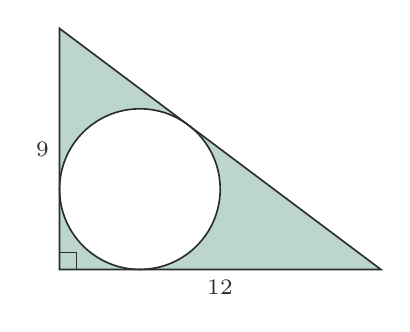
\begin{tikzpicture}[line width=0.6pt,ink,every node/.style={font=\footnotesize}]
\fill[accent!28] (0.000mm,0.000mm) -- (40.800mm,0.000mm) -- (0.000mm,30.600mm) -- cycle;
\filldraw[fill=white] (10.200mm,10.200mm) circle (10.200mm);
\draw (0.000mm,0.000mm) -- (40.800mm,0.000mm) -- (0.000mm,30.600mm) -- cycle;
\draw[ink,line width=0.4pt] (2.200mm,0.000mm) -- (2.200mm,2.200mm) -- (0.000mm,2.200mm);
\node[left] at (0.000mm,15.300mm) {$9$};
\node[below] at (20.400mm,0.000mm) {$12$};
\end{tikzpicture}}\immediate\write\mw{incircle \the\wd\figsave\space\the\ht\figsave\space\the\dp\figsave}
\sbox{\figsave}{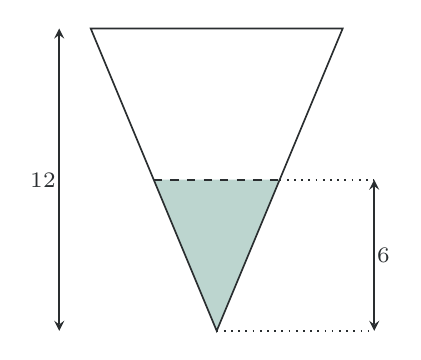
\begin{tikzpicture}[line width=0.6pt,ink,every node/.style={font=\footnotesize}]
\fill[accent!28] (0.000mm,0.000mm) -- (-8.000mm,19.200mm) -- (8.000mm,19.200mm) -- cycle;
\draw (0.000mm,0.000mm) -- (-16.000mm,38.400mm) -- (16.000mm,38.400mm) -- cycle;
\draw[dashed] (-8.000mm,19.200mm) -- (8.000mm,19.200mm);
\draw[<->,>=stealth] (-20.000mm,0.000mm) -- (-20.000mm,38.400mm) node[midway,left,inner sep=1pt] {$12$};
\draw[<->,>=stealth] (20.000mm,0.000mm) -- (20.000mm,19.200mm) node[midway,right,inner sep=1pt] {$6$};
\draw[dotted] (8.000mm,19.200mm) -- (20.000mm,19.200mm);
\draw[dotted] (0.000mm,0.000mm) -- (20.000mm,0.000mm);
\end{tikzpicture}}\immediate\write\mw{conewater \the\wd\figsave\space\the\ht\figsave\space\the\dp\figsave}
\sbox{\figsave}{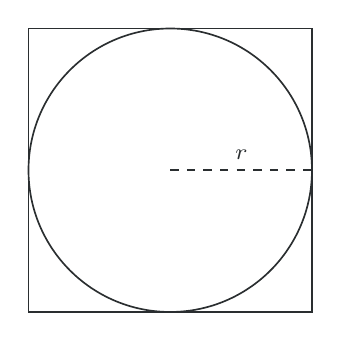
\begin{tikzpicture}[line width=0.6pt,ink,every node/.style={font=\footnotesize}]
\draw (-18.000mm,0.000mm) rectangle (18.000mm,36.000mm);
\draw (0.000mm,18.000mm) circle (18.000mm);
\draw[dashed] (0.000mm,18.000mm) -- (18.000mm,18.000mm);
\node[above=0pt] at (9.000mm,18.000mm) {$r$};
\end{tikzpicture}}\immediate\write\mw{spherecyl \the\wd\figsave\space\the\ht\figsave\space\the\dp\figsave}
\sbox{\figsave}{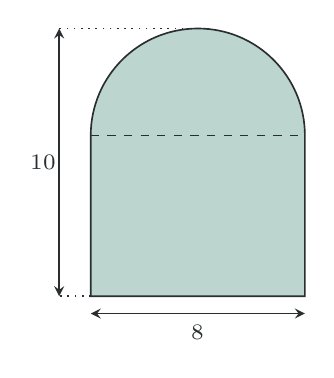
\begin{tikzpicture}[line width=0.6pt,ink,every node/.style={font=\footnotesize}]
\fill[accent!28] (-13.600mm,0.000mm) -- (13.600mm,0.000mm) -- (13.600mm,20.400mm) arc[start angle=0,end angle=180,radius=13.600mm] -- cycle;
\draw (-13.600mm,0.000mm) -- (13.600mm,0.000mm) -- (13.600mm,20.400mm) arc[start angle=0,end angle=180,radius=13.600mm] -- cycle;
\draw[dashed] (-13.600mm,20.400mm) -- (13.600mm,20.400mm);
\draw[<->,>=stealth] (-17.600mm,0.000mm) -- (-17.600mm,34.000mm) node[midway,left,inner sep=1pt] {$10$};
\draw[dotted] (-13.600mm,0.000mm) -- (-17.600mm,0.000mm); \draw[dotted] (0.000mm,34.000mm) -- (-17.600mm,34.000mm);
\draw[<->,>=stealth] (-13.600mm,-2.200mm) -- (13.600mm,-2.200mm) node[midway,below=0.5pt] {$8$};
\end{tikzpicture}}\immediate\write\mw{silo \the\wd\figsave\space\the\ht\figsave\space\the\dp\figsave}
\sbox{\figsave}{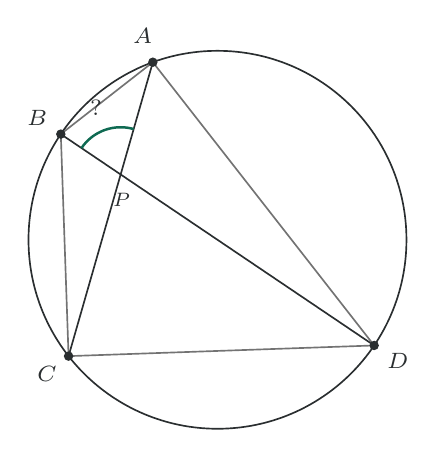
\begin{tikzpicture}[line width=0.6pt,ink,every node/.style={font=\footnotesize}]
\draw (0.000mm,0.000mm) circle (24.000mm);
\draw (-8.208mm,22.553mm) -- (-18.912mm,-14.776mm); \draw (-19.897mm,13.421mm) -- (19.897mm,-13.421mm);
\draw[black!55] (-8.208mm,22.553mm) -- (-19.897mm,13.421mm) -- (-18.912mm,-14.776mm) -- (19.897mm,-13.421mm) -- cycle;
\draw[accent,line width=0.9pt] (-10.643mm,14.062mm) arc[start angle=74.000,end angle=146.000,radius=6mm];
\node[inner sep=0pt] at (-15.375mm,16.752mm) {$?$};
\fill[ink] (-8.208mm,22.553mm) circle (0.6mm); \node[inner sep=0pt] at (-9.440mm,25.936mm) {$A$};
\fill[ink] (-19.897mm,13.421mm) circle (0.6mm); \node[inner sep=0pt] at (-22.881mm,15.434mm) {$B$};
\fill[ink] (-18.912mm,-14.776mm) circle (0.6mm); \node[inner sep=0pt] at (-21.749mm,-16.992mm) {$C$};
\fill[ink] (19.897mm,-13.421mm) circle (0.6mm); \node[inner sep=0pt] at (22.881mm,-15.434mm) {$D$};
\node[inner sep=0pt,xshift=0pt] at (-12.297mm,5.094mm) {\scriptsize $P$};
\end{tikzpicture}}\immediate\write\mw{chords \the\wd\figsave\space\the\ht\figsave\space\the\dp\figsave}
\sbox{\figsave}{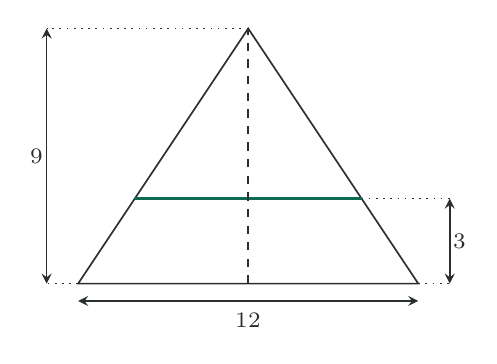
\begin{tikzpicture}[line width=0.6pt,ink,every node/.style={font=\footnotesize}]
\draw (-21.600mm,0.000mm) -- (21.600mm,0.000mm) -- (0.000mm,32.400mm) -- cycle;
\draw[accent,line width=1.2pt] (-14.400mm,10.800mm) -- (14.400mm,10.800mm);
\draw[dashed] (0.000mm,0.000mm) -- (0.000mm,32.400mm);
\draw[<->,>=stealth] (-21.600mm,-2.200mm) -- (21.600mm,-2.200mm) node[midway,below=0.5pt] {$12$};
\draw[<->,>=stealth] (-25.600mm,0.000mm) -- (-25.600mm,32.400mm) node[midway,left,inner sep=1pt] {$9$};
\draw[dotted] (-21.600mm,0.000mm) -- (-25.600mm,0.000mm); \draw[dotted] (0.000mm,32.400mm) -- (-25.600mm,32.400mm);
\draw[<->,>=stealth] (25.600mm,0.000mm) -- (25.600mm,10.800mm) node[midway,right,inner sep=1pt] {$3$};
\draw[dotted] (14.400mm,10.800mm) -- (25.600mm,10.800mm);
\draw[dotted] (21.600mm,0.000mm) -- (25.600mm,0.000mm);
\end{tikzpicture}}\immediate\write\mw{pyramid \the\wd\figsave\space\the\ht\figsave\space\the\dp\figsave}
\sbox{\figsave}{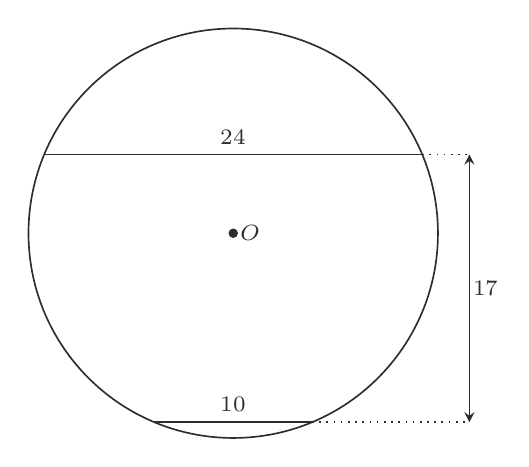
\begin{tikzpicture}[line width=0.6pt,ink,every node/.style={font=\footnotesize}]
\draw (0.000mm,0.000mm) circle (26.000mm);
\draw (-24.000mm,10.000mm) -- (24.000mm,10.000mm); \draw (-10.000mm,-24.000mm) -- (10.000mm,-24.000mm);
\fill[ink] (0.000mm,0.000mm) circle (0.6mm); \node[right,inner sep=1.5pt,xshift=1pt] at (0.000mm,0.000mm) {$O$};
\draw[dotted] (24.000mm,10.000mm) -- (30.000mm,10.000mm); \draw[dotted] (10.000mm,-24.000mm) -- (30.000mm,-24.000mm);
\draw[<->,>=stealth] (30.000mm,-24.000mm) -- (30.000mm,10.000mm) node[midway,right,inner sep=1pt] {$17$};
\node[above] at (0.000mm,10.000mm) {$24$};
\node[above] at (0.000mm,-24.000mm) {$10$};
\end{tikzpicture}}\immediate\write\mw{parallel \the\wd\figsave\space\the\ht\figsave\space\the\dp\figsave}
\immediate\closeout\mw
\end{document}